\documentclass[10pt]{article}
\usepackage[polish]{babel}
\usepackage[utf8]{inputenc}
\usepackage[T1]{fontenc}
\usepackage{amsmath}
\usepackage{amsfonts}
\usepackage{amssymb}
\usepackage[version=4]{mhchem}
\usepackage{stmaryrd}
\usepackage{graphicx}
\usepackage[export]{adjustbox}
\graphicspath{ {./images/} }

\title{GIMNAZJUM }

\author{}
\date{}


\begin{document}
\maketitle
\begin{enumerate}
  \item Środki kolejnych boków pięciokąta wypukłego połączono odcinkami i otrzymano łamaną o długośsi \(7,3 \mathrm{~cm}\). Oblicz sumę długości wszystkich przekątnych tego pięciokąta.
  \item Wykaż, że \(\frac{1}{1 \cdot 2}+\frac{1}{2 \cdot 3}+\frac{1}{3 \cdot 4}+\cdots+\frac{1}{n(n+1)}=\frac{n}{n+1}\)\\
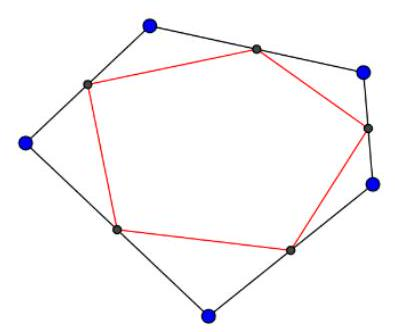
\includegraphics[max width=\textwidth, center]{2024_11_21_867f497540a78012e3fbg-1}
  \item Wykazać, że spośród dowolnych 37 liczb całkowitych niepodzielnych przez siedem można wybrać siedem liczb, których suma jest podzielna przez siedem.
\end{enumerate}

\section*{LICEUM}
\begin{enumerate}
  \item Udowodnij, że \(\underbrace{22 \ldots 2}_{n}+\underbrace{33 \ldots 3^{2}}_{n}=\underbrace{11 \ldots 1}_{2 n}\)
  \item Dany jest równoległobok \(A B C D\) oraz równoległobok \(A C E F\), którego bok \(E F\) przechodzi przez punkt \(D\). Udowodnij, że te równoległoboki mają jednakowe pola.
  \item Liczby rzeczywiste \(a\) i \(b\) spełniają równość
\end{enumerate}

\[
\frac{2 a}{a+b}+\frac{b}{a-b}=2
\]

Jakie wartości może przyjmować ułamek \(\frac{3 a-b}{a+5 b}\) ?


\end{document}